\documentclass[submit]{harvardml}

% Put in your full name and email address.
\name{Timothy Kang}
\email{tkang01@college.harvard.edu}

% List any people you worked with.
\collaborators{%
  }

% You don't need to change these.
\course{CS181-S16}
\assignment{Assignment \#1}
\duedate{5:00pm February 5, 2016}

\usepackage[OT1]{fontenc}
\usepackage[colorlinks,citecolor=blue,urlcolor=blue]{hyperref}
\usepackage[pdftex]{graphicx}
\usepackage{subfig}
\usepackage{fullpage}
\usepackage{palatino}
\usepackage{mathpazo}
\usepackage{amsmath}
\usepackage{amssymb}
\usepackage{color}
\usepackage{todonotes}
\usepackage{listings}
\usepackage{common}
\usepackage{enumerate}

\usepackage[mmddyyyy,hhmmss]{datetime}

\definecolor{verbgray}{gray}{0.9}

\lstnewenvironment{csv}{%
  \lstset{backgroundcolor=\color{verbgray},
  frame=single,
  framerule=0pt,
  basicstyle=\ttfamily,
  columns=fullflexible}}{}
 

\begin{document}
\begin{center}
{\Large Homework 1: Linear Regression}\\
\end{center}
You should submit your answers as a PDF via the Canvas course website.  There is a mathematical component and a programming component to this homework.You may collaborate with others, but are expected to list collaborators, and write up your problem sets individually.\\

\noindent
Please type your solutions after the corresponding problems using this \LaTeX\ template, and start each problem on a new page.\\

%%%%%%%%%%%%%%%%%%%%%%%%%%%%%%%%%%%%%%%%%%%%%
% Problem 1
%%%%%%%%%%%%%%%%%%%%%%%%%%%%%%%%%%%%%%%%%%%%%
\begin{problem}[Centering and Ridge Regression, 7pts]
%\subsection*{1. Centering and Ridge Regression [7pts]}

Consider a data set in which each data input vector $\boldx \in \mathbb{R}^n$ is
centered, meaning $\forall \boldx, \sum_i x_i = 0$. Let $\boldX \in
\mathbb{R}^{n \times m}$ be the input matrix, the columns of which are the input
vectors. Let $\lambda$ be a positive constant. We define:

$$J(\boldw, w_0) = (\boldy - \boldX \boldw - w_0 {\bf 1 })^T (\boldy - \boldX
\boldw - w_0 {\bf 1 }) + \lambda \boldw^T \boldw$$

\begin{itemize}
  \item[(a)] Compute the gradient of $J(\boldw, w_0)$ with respect to $w_0$.
    Simplify as much as you can for full credit.
  \item[(b)] Compute the gradient of $J(\boldw, w_0)$ with respect to $\boldw$.
    Simplify as much as you can for full credit. Make sure to give your answer
    in matrix form.
  \item[(c)] Suppose that $\lambda > 0$. Knowing that $J$ is a convex function
    of its arguments, conclude that a global optimizer of
    $J(\boldw, w_0)$ is
    \begin{align}
      w_0 &= \frac{1}{n} \sum_i y_i \\
      \boldw &= (\boldX^T \boldX + \lambda \boldI)^{-1} \boldX^T \boldy
    \end{align}
    Before taking the inverse of a matrix, prove that it is invertible.
\end{itemize}
\end{problem}

\subsubsection*{Solution}
\begin{enumerate}[(a)]
	\item We begin by noting that $(\textbf{y} - \textbf{X}\textbf{w}- w_0\textbf{1})^T$ is a $1 \times n$ matrix, and that $(\textbf{y} - \textbf{X}\textbf{w}- w_0\textbf{1})$ is an $n \times 1$ matrix. This indicates that the product of 
	these two matrices is a $1 \times 1$ matrix. If we consider the example of the vector $[1 \quad 2 \quad 3]$ times
	its transpose, we would have the $1 \times 1$ matrix $[1^2 +2^2+3^2]$. We observe a similar result when we multiply $(\textbf{y} - \textbf{X}\textbf{w}- w_0\textbf{1})$ by its transpose: We would get a $1 \times 1$ matrix
	with entries
		$$[(y_1-\textbf{x}_1\textbf{w} - w_0)^2 + \dots +  (y_n-\textbf{x}_n\textbf{w} - w_0)^2 ]$$
	This is equivalent to the expression
		$$\sum_{i} (y_i - \textbf{x}_1\textbf{w} - w_0)^2 $$	
	When we take the gradient w.r.t. $w_0$, we apply the chain rule and ignore the last term in $J(\textbf{w},w_0)$
	since it does not contain $w_0$
		\begin{align*}
			\nabla_{w_0} J(\textbf{w},w_0) &= -2 \sum_{i} (y_i - \textbf{x}_1\textbf{w} - w_0) \\
			&= -2 \left(\sum_i y_i - \sum_i \textbf{x}_i\textbf{w} - \sum_i w_0\right) \\
			&= -2 \left(\sum_i y_i - nw_0\right) \\
			&= \boxed{2\left(nw_0-\sum_i y_i  \right)}
		\end{align*}	
	We set the $\sum_i \textbf{x}_i\textbf{w}$ term equal to 0 because we use the fact that $\textbf{x}$ is centered $\forall \textbf{x}$, 
	which by definition includes $\textbf{x}$ multiplied by a factor - in this case, the coordinate of $w_0$. 
	\item  Before taking the gradient, we expand the polynomial and use properties of matrix transposes to 
	simplify. Furthermore, we make use
	of the identity $\nabla_\textbf{z} \textbf{z}^T \textbf{A} \textbf{z} =  (\textbf{A}+ \textbf{A}^T)\textbf{z}$
		\begin{align*}
			J(\textbf{w},w_0) &= \textbf{y}^T\textbf{y} - \textbf{y}^T\textbf{X}\textbf{w} - \textbf{y}^Tw_0\textbf{1} - \textbf{w}^T\textbf{X}^T\textbf{y} +\textbf{w}^T\textbf{X}^T\textbf{X}\textbf{w} \\
			&+ \textbf{w}^T\textbf{X}^Tw_0\textbf{1} -  \textbf{1}^Tw_0\textbf{y} + \textbf{1}^Tw_0\textbf{X}\textbf{w} + \textbf{1}^Tw_0^2\textbf{1} + \lambda\textbf{w}^T\textbf{w} \\
			\nabla_\textbf{w} J(\textbf{w},w_0) &=-2\textbf{X}^T\textbf{y} + \textbf{X}^T\textbf{X}\textbf{w} + 2\lambda\textbf{I}\textbf{w} \\ 
			&= \boxed{-2\textbf{X}^T\textbf{y} +2 \textbf{X}^T\textbf{X}\textbf{w} +2 \lambda\textbf{I}\textbf{w}}
		\end{align*}
	We do not include the $ \textbf{1}^Tw_0\textbf{X}\textbf{w}$ term and its transpose because they both 
	result in $1 \times 1$ matrices with elements of the form 
		$$\textbf{x}_1\textbf{w}w_0 + \dots +\textbf{x}_n\textbf{w}w_0$$ 
	(transpose of $1 \times 1$ matrix is itself) \\
	Using the same reasoning as part (a), we set this term equal to 0 because it results in a summation of the form
		$$w_0 \sum_i \textbf{x}_i\textbf{w}$$ 		
	\item  
		\begin{itemize}
			\item When we set the answer from (a) equal to zero (optimization entails setting the first 
				derivative equal to 0), we get
					\begin{align*}
						2\left(nw_0-\sum_i y_i  \right) &= 0 \\
						nw_0 &= \sum_i y_i \\
						w_0 &= \frac{1}{n} \sum_i y_i
					\end{align*}
			\item When we do the same for the answer for part (b), we get
					\begin{align*}
						-2\textbf{X}^T\textbf{y} +2 \textbf{X}^T\textbf{X}\textbf{w} +2 \lambda\textbf{I}\textbf{w} &= 0\\
						(\textbf{X}^T\textbf{X} + \lambda\textbf{I})\textbf{w} &= \textbf{X}^T\textbf{y} \\ 
						\textbf{w} &= (\textbf{X}^T\textbf{X} + \lambda\textbf{I})^{-1} \textbf{X}^T\textbf{y}
					\end{align*}
				We prove that $\textbf{X}^T\textbf{X} + \lambda\textbf{I}$ is invertible by demonstrating that 
				it is positive definite $\forall v$
					\begin{align*}
						v^T(\textbf{X}^T\textbf{X} + \lambda\textbf{I})v &= (v^T\textbf{X}^T\textbf{X} + \lambda v^T\textbf{I})v  \\
						&= v^T\textbf{X}^T\textbf{X}v + \lambda v^T\textbf{I}v\\
						&= (\textbf{X}v)^T(\textbf{X}v) + \lambda(v^T v) \\
						&= \sum(\text{values})^2 + \lambda \sum(\text{values})^2 > 0
					\end{align*}
				Therefore, $\textbf{X}^T\textbf{X} + \lambda\textbf{I}$ is invertible. 	
		\end{itemize}
\end{enumerate}










%%%%%%%%%%%%%%%%%%%%%%%%%%%%%%%%%%%%%%%%%%%%%
% Problem 2
%%%%%%%%%%%%%%%%%%%%%%%%%%%%%%%%%%%%%%%%%%%%%
\newpage
%\subsection*{2. Priors and Regularization [7pts]}
\begin{problem}[Priors and Regularization,7pts]
Consider the Bayesian linear regression model given in Bishop 3.3.1. The prior is
\begin{align*}
p(\boldw \given \alpha) = \mathcal{N}(\boldw \given \bold0, \alpha^{-1}\ident ),
\end{align*}
where $\alpha$ is the precision parameter that controls the variance of the Gaussian prior.  The likelihood can be written as
\begin{align*}
p(\boldt \given \boldw) &= \prod_{n=1}^N \mcN(t_n \given \boldw^\trans \bphi(\boldx_n), \beta^{-1}),
\end{align*}

Using the fact that the posterior is the product of the prior and the likelihood (up to a normalization constant), show that maximizing the log posterior (i.e., $\ln p(\boldw \given \boldt)= \ln p(\boldw | \alpha) + \ln p(\boldt \given \boldw)$) is equivalent to minimizing the regularized error term given by ${E_D(\boldw) + \lambda E_W(\boldw)}$ with 
\begin{align*}
E_D(\boldw) &= \frac{1}{2}\sum_{n = 1}^N (t_n - \boldw^\trans \bphi(\boldx_n))^2 \\
E_W(\boldw) &= \frac{1}{2}\boldw^\trans \boldw
\end{align*} 

Do this by writing $\ln p(\boldw \given \boldt)$ as a function of $E_D(\boldw)$ and $E_W(\boldw)$, dropping constant terms if necessary.  Conclude that maximizing this posterior is equivalent to minimizing the regularized error term given by $E_D(\boldw) + \lambda E_W(\boldw)$. (Hint: take $\lambda = \alpha/\beta$)
\end{problem}
\subsubsection*{Solution}

We begin by observing that $p(\textbf{w}|\alpha)$ is a multivariate normal distribution of dimensionality $D$ with mean $\textbf{0}$ and covariance matrix $\alpha^{-1}\textbf{I}$. With this in mind, we plug in the appropriate values into the distribution for a multivariate normal (as given in the math review sheet).
	\begin{align*}
		p(\textbf{w}|\alpha) &= \frac{1}{\sqrt{2\pi^D\text{det}(\alpha^{-1}\textbf{I})}}e^{-\frac{1}{2}\textbf{w}^T(\alpha^{-1}\textbf{I})^{-1}{\textbf{w}}} \\
		\text{ln}(p(\textbf{w}|\alpha)) &= -\frac{1}{2}\textbf{w}^T\textbf{I}^{-1}\alpha\textbf{w} + \text{ln}\left(\frac{1}{\sqrt{2\pi^D\text{det}(\alpha^{-1}\textbf{I})}}\right)\\
		&= -\frac{1}{2}\textbf{w}^T\textbf{w}\alpha + \text{constant} \\ 
		&= -\alpha E_W(\textbf{w}) + \text{constant}
	\end{align*}
We also observe that $p(\textbf{t}|\textbf{w})$ is a product of $N$ univariate normal distributions with mean $\textbf{w}^T\boldsymbol{\phi}(\textbf{x}_n)$ and variance $\beta^{-1}$. We plug the values into the distribution for the univariate normal.
	\begin{align*}
		p(\boldsymbol{t}|\boldsymbol{w}) &= \prod^N_{n=1} N(t_n | \textbf{w}^T\boldsymbol{\phi}(\textbf{x}_n), \beta^{-1}) \\
		&= \frac{1}{\sqrt{2\pi\beta^{-1}}}\prod^N_{n=1}  e^{-\frac{1}{2\beta^{-1}} (t_n - \textbf{w}^T\boldsymbol{\phi}(\textbf{x}_n))^2}\\
		\text{ln}(p(\boldsymbol{t}|\boldsymbol{w})) &= -\frac{1}{2}\sum^N_{n=1} (t_n - \textbf{w}^T\boldsymbol{\phi}(\textbf{x}_n))^2 + \ln\left( \frac{1}{\sqrt{2\pi\beta^{-1}}} \right)\\
		&= - \beta E_D(\textbf{w}) + \text{constant} 
	\end{align*}
Therefore, when we maximize the posterior, we are really maximizing
	$$-(\alpha E_W(\textbf{w}) + \beta E_D(\textbf{w})) + \text{constant}$$
And if we remember that maximizing a function is the same as minimizing its negative, then it becomes clear that  this is the same as minimizing 
	$$E_D(\textbf{w}) + \lambda E_W(\textbf{w})$$
where $\lambda  = \frac{\alpha}{\beta}$	















%%%%%%%%%%%%%%%%%%%%%%%%%%%%%%%%%%%%%%%%%%%%%
% Problem 3
%%%%%%%%%%%%%%%%%%%%%%%%%%%%%%%%%%%%%%%%%%%%%
\newpage
\subsection*{3. Modeling Changes in Congress [10pts]}
 The objective of this problem is to learn about linear regression with basis
 functions by modeling the average age of the US Congress. The file
 \verb|congress-ages.csv| contains the data you will use for this problem.  It
 has two columns.  The first one is an integer that indicates the Congress
 number. Currently, the 114th Congress is in session. The second is the average
 age of that members of that Congress.  The data file looks like this:
\begin{csv}
congress,average_age
80,52.4959
81,52.6415
82,53.2328
83,53.1657
84,53.4142
85,54.1689
86,53.1581
87,53.5886
\end{csv}
and you can see a plot of the data in Figure~\ref{fig:congress}.

\begin{figure}[h]
\centering
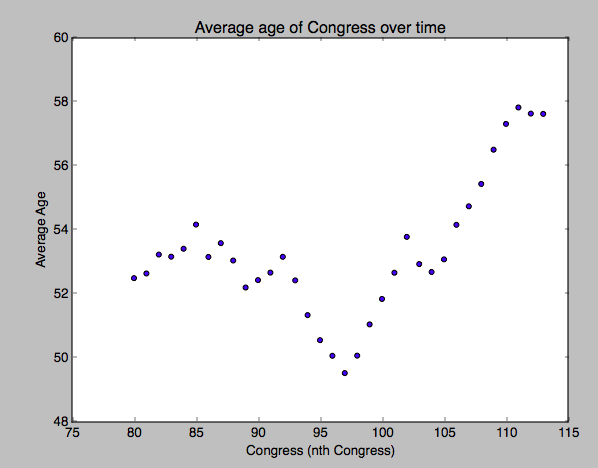
\includegraphics[width=0.8\textwidth]{congress-ages}
\caption{Average age of Congress.  The horizontal axis is the Congress number, and the vertical axis is the average age of the congressmen.}
\label{fig:congress}
\end{figure}

\begin{problem}[Modeling Changes in Congress, 10pts]
Implement basis function regression with ordinary least squares with the above
data. Some sample Python code is provided in \verb|linreg.py|, which implements
linear regression.  Plot the data and regression lines for the simple linear
case, and for each of the following sets of basis functions:
\begin{itemize}
	\item[(a)] $\phi_j(x) = x^j$ for $j=1, \ldots, 7$
	\item[(b)] $\phi_j(x) = x^j$ for $j=1, \ldots, 3$
	\item[(c)] $\phi_j(x) = \sin\{ x / j \}$ for $j=1, \ldots, 4$
	\item[(d)] $\phi_j(x) = \sin\{ x / j \}$ for $j=1, \ldots, 7$
	\item[(e)] $\phi_j(x) = \sin\{ x / j \}$ for $j=1, \ldots, 20$
\end{itemize}
  In addition to the plots, provide one or two sentences for each, explaining
  whether you think it is fitting well, overfitting or underfitting.  If it does
  not fit well, provide a sentence explaining why. A good fit should capture the
  most important trends in the data.
	\end{problem}

\subsubsection*{Solution}

\begin{enumerate}[(a)]
	\item 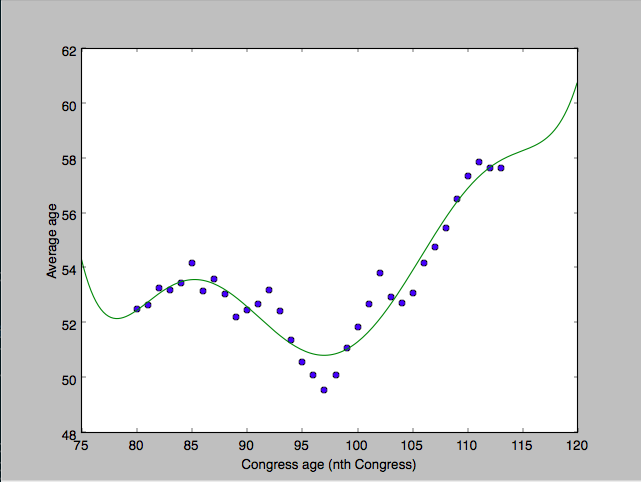
\includegraphics[scale = 0.3]{./a} \\
		This regression is an overall good fit, as it tracks the trends in the data relatively accurately without 
		major deviations, and it does not seem to be affected by potential outliers, such as those around 
		the drop from 95-100 (on the x-axis).
	\item 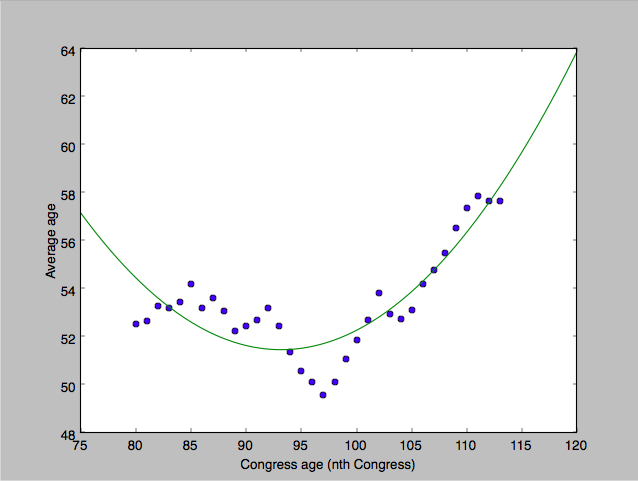
\includegraphics[scale = 0.3]{./b} \\
		This regression under-fits the data, as it fails to account for most of the trends in the data, such as the 
		peaks from 85-93 (on the x-axis) and the drop from 95-100 (on the x-axis).
	\item 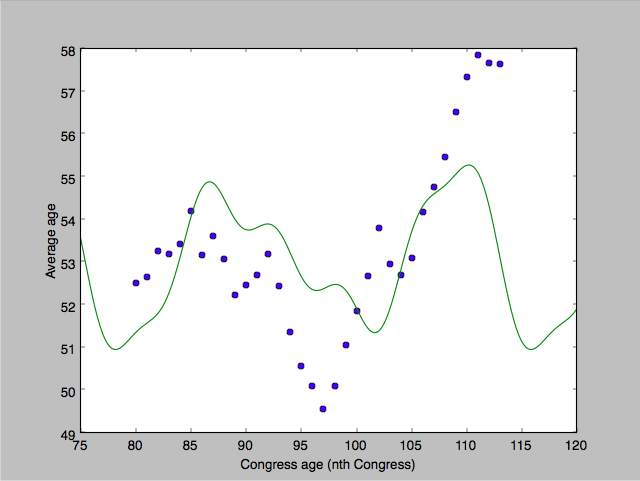
\includegraphics[scale = 0.3]{./c}\\	
		This one also under-fits the data because it does not follow the trends in the data. For example, it 
		completely misses the peak from 100 - 104 (on the x-axis) and most of the drop from 95-100.
	\item 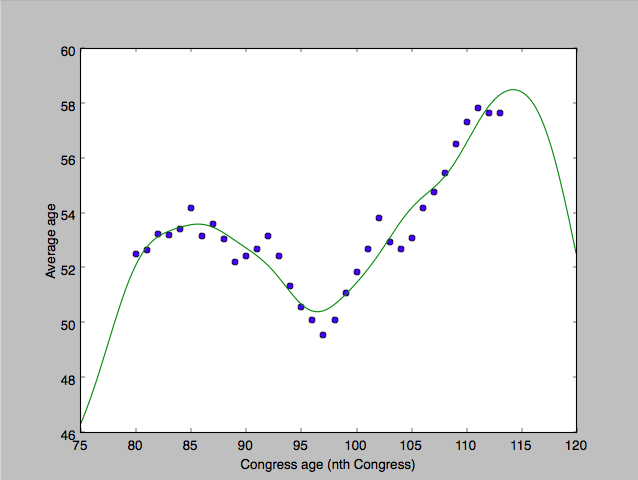
\includegraphics[scale = 0.3]{./d} \\
		While this one seems to be a good fit (it is mostly similar to the regression from (a)), it still overfits 
		the data by following the trends too closely. For example, the drop from 95 - 100 may constitute 
		noise, but the regression follows the trend almost perfectly. 
	\item 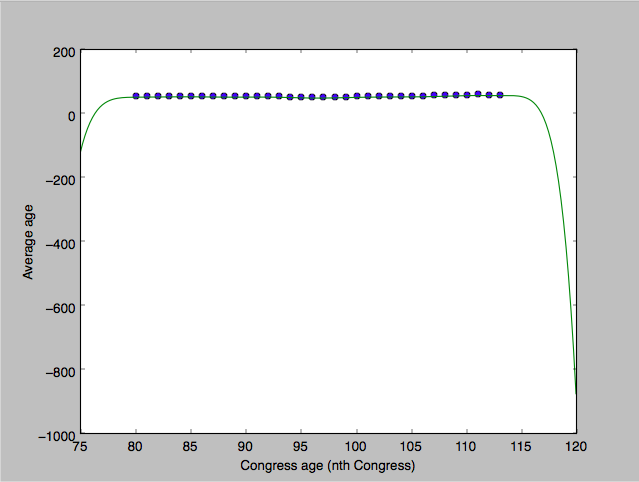
\includegraphics[scale = 0.3]{./e}\\
		This regression heavily overfits the data. At this point, the regression is tracking not only the trends in the
		data but also all of the noise, as all of the points fit on the regression. 
\end{enumerate}










\newpage
\begin{problem}[Calibration, 1pt]
Approximately how long did this homework take you to complete?
\end{problem}
\textbf{Answer:}
Roughly 3 hours. Most of it was remembering my linear algebra theory for problem 1. 

\end{document}
